\documentclass[twoside,a4paper]{report}

\usepackage[pdftex]{graphicx}
\usepackage{textcomp}
\usepackage{titlesec}
\titleformat{\chapter}[display]
  {\normalfont\bfseries}{}{0pt}{\huge}
\usepackage{lipsum}
\usepackage{wrapfig}
\usepackage[utf8]{inputenc}
\usepackage[polish]{babel}
\usepackage[T1]{fontenc}
\usepackage[fit]{truncate}
\usepackage{array}
\usepackage{float}
\usepackage{anysize}
\usepackage{enumitem}
\usepackage[font=small,labelfont=bf]{caption}
\usepackage{url}
\usepackage{hyperref}
\usepackage{csquotes}
\usepackage[
sorting=none
]{biblatex}
\addbibresource{bibliografia.bib}
\usepackage{listings}
\usepackage{fancyhdr}
\usepackage{multirow}
\usepackage{tabularx}
\usepackage{indentfirst}
\newcolumntype{C}{>{\centering\arraybackslash}X}

\newcommand*{\noaddvspace}{\renewcommand*{\addvspace}[1]{}}
\addtocontents{lof}{\protect\noaddvspace}

\pagestyle{fancy}
\fancyhf{}

\graphicspath{{img}}

\renewcommand{\lstlistlistingname}{Spis listingów}

\renewcommand{\chaptermark}[1]{\markboth{#1}{}}
\renewcommand{\sectionmark}[1]{\markright{\thesection\ #1}}
\renewcommand{\headrulewidth}{0.5pt}
\renewcommand{\footrulewidth}{0pt}

\fancyhead[LE,RO]{\bfseries\thepage}
\fancyhead[LO]{\nouppercase{\bfseries{\truncate{.95\headwidth}{\rightmark}}}}
\fancyhead[RE]{\nouppercase{\bfseries{\truncate{.95\headwidth}{\leftmark}}}}

\linespread{1.5}

\parskip0.05in

\marginsize{3.5cm}{2.5cm}{2.5cm}{2.5cm}
\fancyhfoffset[E,O]{0pt}

% --------------------------------------------------------------------------------

\begin{document}

% allows useg @ as a @ not as special character
% required for macro redefinition
\makeatletter

% parameters definition
% they cannot conflict with other
% like bibteh attributes etc.
\def\tytul#1{\def\@tytul{#1}}
\def\promotor#1{\def\@promotor{#1}}
\def\miasto#1{\def\@miasto{#1}}
\def\studies#1{\def\@studies{#1}}
\def\descr#1{\def\@descr{#1}}
\def\indeks#1{\def\@indeks{#1}}
\def\dept#1{\def\@dept{#1}}
\def\spec#1{\def\@spec{#1}}

\def\maketitle{
    %removal of header
    \keepXColumns
    \thispagestyle{empty}%
    \begin{center}
        \begin{tabularx}{\textwidth}{CcC}
            \multirow{4}{*}{
\includegraphics[height=2.35cm]{img/logo_pg.png}}
          & \textsc{\textbf{Politechnika Gdańska}} &
          \multirow{4}{*}{
\includegraphics[height=2.35cm]{img/logo_eti.png}}
       \\ & & \\
          & \textsc{\textbf{Wydział Elektroniki, }}& \\
          & \textsc{\textbf{Telekomunikacji i Informatyki }}& \\
        \end{tabularx}
    \end{center}
    \begin{center}
        \begin{tabularx}{\textwidth}{XX}
            \textbf{Katedra:} & \@dept\\
                              &\\
            \textbf{Imię i nazwisko dyplomanta:} & \@author\\
                                                 &\\
            \textbf{Nr albumu:} & \@indeks\\
                                &\\
            \textbf{Forma i poziom studiów:} & \@studies\\
                                             &\\
            \textbf{Kierunek studiów:} & Informatyka\\
                                       &\\
            \textbf{Specjalność:} & \@spec
        \end{tabularx}
    \end{center}
    \begin{center}
        \Large{\textbf{Praca dyplomowa magisterska}}
    \end{center}
    \vspace{1cm}
    \begin{tabular}{l}
        \textbf{Temat pracy:} \\ \@tytul\\
        \\
        \textbf{Title of thesis:} \\ \@title\\
        \\
        \textbf{Opiekun pracy:} \\ \@promotor\\
        \\
        \textbf{Data ostatecznego zatwierdzenia raportu podobieństw w JSA:} TBA
    \end{tabular}
    \vspace*{\stretch{6}}
    \begin{center}
        \@miasto, \@date
    \end{center}

}

%restore @ sign
\makeatother

\cleardoublepage


\tytul{Wykorzystanie języka Elm do tworzenia aplikacji frontendowych.}
\title{Programming the front-end applications with Elm language.}
\author{Marcin Jurczak}
\date{2022}
\miasto{Gdańsk}
\promotor{dr\ inż.\ Krzysztof Manuszewski}
\studies{Stacjonarne jednolite studia magisterskie}
\indeks{171641}
\dept{Algorytmów i Modelowania Systemów}
\spec{Algorytmów i Technologii Internetowych}

\maketitle

% --------------------------------------------------------------------------------

\chapter*{Streszczenie}
\noindent
Celem niniejszej pracy magisterskiej było stworzenie front-end'owej aplikacji internetowej z wykorzystaniem funkcyjnego języka Elm, porównanie tejże technologii z istniejącymi, bardziej powszechnymi rozwiązaniami tego typu, a także przygotowanie instrukcji laboratoryjnej, która mogłaby zostać wykorzystana w ramach zajęć \textit{Współczesne Aplikacje Programowania Funkcyjnego} przeprowadzanych na Wydziale Elektroniki, Telekomunikacji i Informatyki Politechniki Gdańskiej.
Wytworzona aplikacja to strona internetowa typu \textit{startpage}, czyli startowa strona przeglądarki, zawierająca najpotrzebniejsze informacje, takie jak czas, pogoda oraz odnośniki do wyszukiwarki i najczęściej odwiedzanych stron.

\textbf{Słowa kluczowe:} Elm, programowanie funkcyjne, wytwarzane aplikacji internetowych

\textbf{Dziedzina nauki i techniki: }Nauki inżynieryjne i techniczne, inżynieria informatyczna.

{\let\clearpage\relax\chapter*{Abstract}}
\noindent
The goal of this master thesis is to use the Elm language to create a front-end web application, comparing this technology to existing, more popular solutions, as well as preparing a lab instruction, which could be used at \textit{Modern applications of functional programming} class at Gdańsk University of Technology’s Faculty of Electronics, Telecommunications and Informatics.
The created application is a \textit{startpage}, meaning a starting page of a web browser consisting of the most useful information, such as time, weather and references to search engine and the most visited websites.

\textbf{Keywords:} Elm, functional programming, web development

\textbf{Field of Science and Technology:} Engineering and Technology, Information engineering.

% --------------------------------------------------------------------------------

\tableofcontents

% --------------------------------------------------------------------------------

\chapter*{Wykaz najważniejszych skrótów}
\begin{tabular}{rl}
    \textbf{CD} &-- ang.~Continuous Deployment, pol.~ciągłe wdrażanie.\\
    \textbf{CI} &-- ang.~Continuous Integration, pol.~ciągła integracja.\\
    \textbf{CSS} &-- ang.~Cascading Style Sheets, pol.~kaskadowe arkusze stylów\\
    \textbf{HTML} &-- ang.~Hypertext Markup Language, pol.~hipertekstowy język znaczników.\\
    \textbf{HTTP} &-- ang.~Hypertext Transfer Protocol, pol.~protokół przesyłania hipertekstu.\\
    \textbf{JSON} &-- ang.~JavaScript Object Notation, pol.~tekstowy format zapisu danych\\
\end{tabular}

% --------------------------------------------------------------------------------

\chapter{Wstęp i cel pracy}
\begin{wrapfigure}{r}{0.25\textwidth}
    \centering
    \centering
    
\includegraphics[width=0.25\textwidth]{elm_logo.png}
    \caption*{Logo Elm'a}\label{elm_logo}
\end{wrapfigure}
Głównym celem niniejszej pracy jest zapoznanie się z funkcyjnym językiem programowania Elm oraz stworzenie przykładowej frontendowej aplikacji internetowej.
Ponadto chciałbym przeprowadzić porównanie tej technologii z innymi, bardziej powszechnie używanymi rozwiązaniami do tworzenia aplikacji internetowych.
Ostatnim celem pracy jest przygotowanie części dydaktycznej w postaci instrukcji laboratoryjnej, która mogłaby zostać potencjalnie wykorzystana w ramach przedmiotu Współczesne Aplikacje Programowania Funkcyjnego, prowadzonego przez mojego promotora, dra inż. Krzysztofa Manuszewskiego.

W drugim rozdziale skupiam się na przedstawieniu technologii powszechnie używanych do tworzenia frontendowych aplikacji internetowych, t.j. React, Angular oraz Vue.
Prezentuję ich zalety i wady względem siebie, a także przedstawiam cechy wyróżniające je między sobą.

Trzeci rozdział poświęcam na wysokopoziomowe wprowadzenie do języka Elm.
Mówię o idei jaka przyświęcała stworzeniu tego języka, jakie są jego potencjalne zastosowania, gdzie sprawdza się najlepiej oraz przedstawiam narzędzia wspomagające tworzenie oprogramowania z użyciem tejże technologii.

W czwartm rozdziale przedstawiam implementację przygotowanej aplikacji frontendowej napisanej w Elm'ie.
Jest to poniekąd rozwinięcie poprzedniego rozdziału, ponieważ głównym celem jest dalej zapoznanie się z Elm'em, jednak tutaj uwagę skupiam na przedstawieniu konkretnych rozwiązań, jakie zostały wykorzystane do osiągniecia wybranego celu.

Piąty rozdział zawiera instrukcję laboratoryjną, w której przeprowadzam czytelnika nieposiadającego żadnego doświadczenia z Elm'em przez proces tworzenia oprogramowania z wykorzystaniem tej technologii, zaczynając od przygotowania środowiska, przez podstawy języka, aż po stworzenie aplikacji frontendowej przedstawionej we wcześniejszym rozdziale.

Szósty rozdział poświęcam na omówienie zagadnień związanych z ciągłą integracją oraz ciągłym wdrażaniem, a także przedstawiam narzędzia wykorzystywane przeze mnie w tym celu podczas tworzenia omawianej aplikacji.
Pokazuję, że Elm nie stanowi przeszkody w wykorzystywaniu tych technologii i całkowicie nadaje się do użytku produkcyjnego.

Ostatni rozdział dotyczy przede wszystkim podsumowania niniejszej pracy magisterskiej.
Przedstawiam produkt dwóch semestrów moich działań oraz wyciągam wnioski na temat Elm'a jako języka przeznaczonego do tworzenia aplikacji frontendowych.

Na końcu dokumentu znajdują się spisy użytych rysunków i listingów, a także bibliografia, która została wykorzystana podczas pracy nad niniejszym dokumentem oraz w czasie zapoznawania się z tematem wytwarzania aplikacji internetowych z wykorzystaniem języka Elm.

% --------------------------------------------------------------------------------

\chapter{Powszechne rozwiązania}

\section{React}
~\cite{react}
~\cite{reactdocs}
\section{Angular}
~\cite{angularjs}
~\cite{angulardocs}
\section{Vue.js}
~\cite{vuejsdocs}
\section{Podobieństwa i różnice}

% --------------------------------------------------------------------------------

\chapter{Elm}
Elm~\cite{elmdocs} jest czysto funkcyjnym językiem programowania przeznaczonym do tworzenia graficznych interfejsów użytkownika.
Powstał w roku 2012 wraz z opublikowaniem przez Evana Czaplickiego pracy~,,Elm: Concurrent FRP for Functional GUIs''~\cite{Czaplicki2012ElmC}.
Podczas jego tworzenia nacisk został położony na użyteczność, wydajność oraz niską podatność na błędy.

\section{Programowanie funkcyjne}

\section{The Elm Architecture}
\begin{figure}[H]
    \centering
    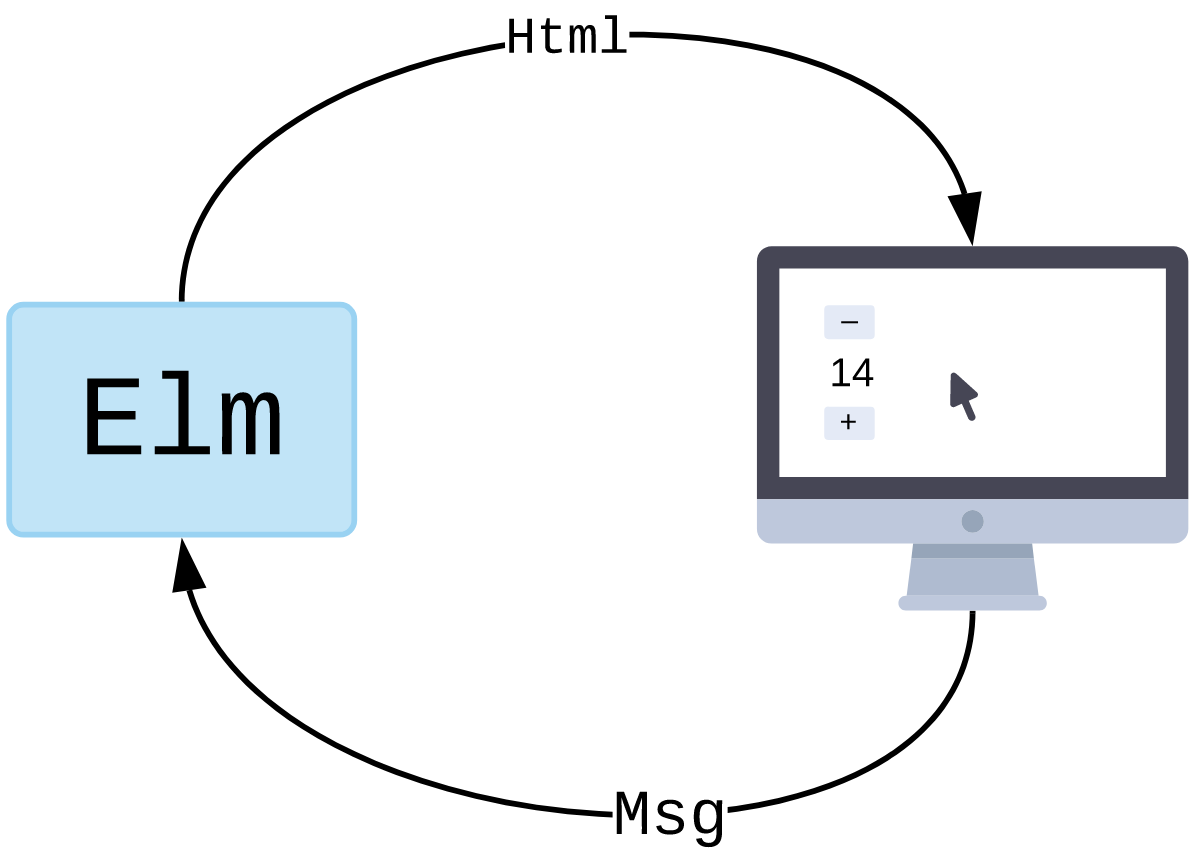
\includegraphics[width=0.6\textwidth]{elm_arch.png}
    \caption{Diagram działania programu w Elm'ie}\label{elm_arch}
\end{figure}

\textit{The Elm Architecture} jest schematem tworzenia interaktywnych aplikacji internetowych lub gier.
Zgodnie z rysunkiem~\ref{elm_arch} typowa aplikacja Elm działa w następujący sposób:
Program generuje pewien kod HTML, który zostaje wyświetlony na ekranie, a następnie komputer zwraca wiadomości informujące o tym co się dzieje, np.~użytkownik wcisnął guzik.

A co się dzieje wewnątrz wspomnianego programu Elm'owego? Zawsze składa się z trzech podstawowych elementów:
\begin{itemize}[noitemsep,topsep=0pt]
    \item Model~-- opisujący stan aplikacji
    \item Update~-- opisujący logikę aplikacji
    \item View~-- opisujący wygląd aplikacji
\end{itemize}
W kolejnych podrozdziałach przedstawiam powyższe elementy architektury Elm'a na podstawie prostego programu, którego zadaniem jest wyświetlenie na ekranie dwóch guzików oraz licznika, który może się zwiększać i zmniejszać, w zależności od tego, który guzik zostanie naciśnięty przez użytkownika.

\subsection{Model}
\begin{minipage}{.50\textwidth}
    Celem modelu jest zdefiniowanie danych w naszej aplikacji.
    W tym przypadku model będzie bardzo prosty~-- jedna wartość całkowitoliczbowa, która będzie mogła zostać zwiększona lub zmniejszona.
\end{minipage}\hfill
\begin{minipage}{.43\textwidth}
    \lstset{frame=single}
    \begin{lstlisting}[caption={\textit{The Elm Architecture} - Model},label=kod:Model]
type alias Model = Int


init : Model
init =
  0
    \end{lstlisting}
\end{minipage}\hfill

\subsection{Update}
\begin{minipage}{.43\textwidth}
    \lstset{frame=single}
    \begin{lstlisting}[caption={\textit{The Elm Architecture} - Update},label=kod:Update]
type Msg
  = Increment
  | Decrement


update : Msg -> Model -> Model
update msg model =
  case msg of
    Increment ->
      model + 1

    Decrement ->
      model - 1
    \end{lstlisting}
\end{minipage}\hfill
\begin{minipage}{.50\textwidth}
    Funkcja \texttt{update} ma za zadanie opisywać jak nasz model będzie się zmieniał w czasie.
    Może odebrać dwa typy wiadomości~-- \textit{Increment} i \textit{Decrement}.
    W wyniku operacji \texttt{update} otrzymujemy nowy, zaktualizowany model.
\end{minipage}\hfill
\subsection{View}
Funkcja \texttt{view} jako argument przyjmuje model i zwraca kod HTML\@.
Wykorzystany został tutaj handler \texttt{onClick}, który po kliknięciu generuje odpowiednią wiadomość.
Znak plusa generuje wiadomość \textit{Increment}, znak minusa \textit{Decrement}.
Wybrana wiadomość trafia do funkcji \texttt{update}.

\lstset{frame=single}
\begin{lstlisting}[caption={\textit{The Elm Architecture} - View},label=kod:View]
view : Model -> Html Msg
view model =
  div []
    [ button [ onClick Decrement ] [ text "-" ]
    , div [] [ text (String.fromInt model) ]
    , button [ onClick Increment ] [ text "+" ]
    ]
\end{lstlisting}
\lstset{frame=none}

\section{Narzędzia}
Platforma Elm jest dostarczana wraz z zestawem narzędzi pozwalających m.in.~na kompilację plików źródłowych czy instalację dodatkowych modułów. Poniżej postaram się opisać większość z tych narzędzi, tj.~dostarczanych przez Elm'a, ale wskazać również te dostarczane przez zewnętrznych twórców, a które znacząco ułatwiły mi pracę z tym językiem.
\begin{center}
    \begin{tabularx}{\textwidth}{llX}
        \texttt{elm repl} &--& otwiera interaktywną sesję programistyczną.\\
        \texttt{elm init} &--& inicjalizuje bieżący katalog jako nowy projekt Elm'a poprzez stworzenie pliku \texttt{elm.json} opisującego projekt i jego zależności, a także tworzy katalog \texttt{src/}, w którym będą znajdowały się pliki \texttt{.elm}.\\
        \texttt{elm reactor} &--& uruchamia serwer deweloperski, który poprzez przeglądarkę pozwala wybrać dany plik źródłowy, skompilować go i sprawdzić jak wygląda po zbudowaniu.\\
        \texttt{elm make} &--& pozwala na kompilację kodu źródłowego do HTML'a lub JavaScript'u. Jest to najbardziej ogólna forma kompilacji, jaką udostępnia Elm, ale jest to niezwykle przydatne narzędzie, kiedy projekt stanie się zbyt skomplikowany na korzystanie z \texttt{elm reactor.}\\
        \texttt{elm install} &--& pozwala instalować paczki dostępne na stronie \url{package.elm-lang.org}, które udostępniają nowe funkcjonalności, jak np.~obsługa plików JSON czy praca z zapytaniami HTTP.\\
        \texttt{elm-live~}\cite{elm-live} &--& //TODO\\
        \texttt{elm-format~}\cite{elm-format} &--& //TODO\\
    \end{tabularx}
\end{center}
% --------------------------------------------------------------------------------

\chapter{Implementacja}
W ramach części praktycznej niniejszej pracy stworzona została aplikacja internetowa typu \textit{startpage}, czyli spersonalizowanej strony startowej przeglądarki zawierającej najpotrzebniejsze i najczęściej używane elementy oraz skróty.
Na potrzeby aplikacji postanowiłem stworzyć cztery moduły:
\begin{itemize}[noitemsep,topsep=0pt]
    \item Cyfrowy zegar wskazujący aktualny czas w strefie czasowej użytkownika
    \item Pogoda w Gdańsku przedstawiona w formie krótkiego opisu oraz temperatury w stopniach Celsjusza
    \item Wyszukiwarka Google
    \item Zakładki zawierające odnośniki do wybranych stron internetowych
\end{itemize}

Powyżej wymienione elementy wykorzystują różne mechanizmy języka, dodatkowe biblioteki Elm'a oraz uwzględniają pracę z najpopularniejszymi sposobami przekazywania informacji w aplikacjach internetowych, takich jak przetwarzanie plików JSON, wysyłanie zapytań HTTP oraz praca z plikami.

W poniższych podrozdziałach skupię się na opisie wymienionych wyżej mechanizmów,

\section{Zegar}

\section{Pogoda}

\section{Wyszukiwarka}

\section{Zakładki}

\section{Dokument hipertekstowy}

\section{Style}

\section{Całość}

% --------------------------------------------------------------------------------

\chapter{Instrukcja laboratoryjna}
W poniższym rozdziale przedstawiam przykładową instrukcję laboratoryjną, która krok po kroku przeprowadza czytelnika przez proces tworzenia aplikacji w Elmie, zaczynając od przygotowania środowiska deweloperskiego, przez podstawy języka wraz z ćwiczeniami pozwalającymi na lepsze zrozumienie składni, aż po stworzenie większej aplikacji frontendowej.

\section{Przygotowanie środowiska}
Pierwszą rzeczą, którą należy się zająć przed rozpoczęciem nowego projektu jest przygotowanie odpowiedniego środowiska deweloperskiego.
Należy upewnić się, że wszystkie narzędzia potrzebne do wykonania pracy są zainstalowane i prawidłowo skonfigurowane.
W przypadku pracy z Elm'em będziemy korzystać przede wszystkim z platformy dostarczanej przez autora, edytora tekstu wspierającego podświetlanie składni, a także innych narzędzi wspomagających proces tworzenia oprogramowania z użyciem tej technologii.

\subsection{Platforma Elm}
Najważniejszą rzeczą, jaka będzie nam potrzebna podczas pracy z Elm'em, będzie platforma języka zawierająca m.in.~takie narzędzia jak kompilator oraz menadżer bibliotek.
Poniżej przedstawiam instukcję instalacji tej platformy na systemach operacyjnych Linux i Windows. Po przejściu tych kroków, w wierszu poleceń należy wykonać instrukcję \texttt{elm}. Jeśli wszystko zostało prawidłowo zainstalowane i skonfigurowane, powinniśmy ujrzeć widok podobny do przedstawionego na rysunku~\ref{elm_output}.
\begin{figure}[H]
    \centering
    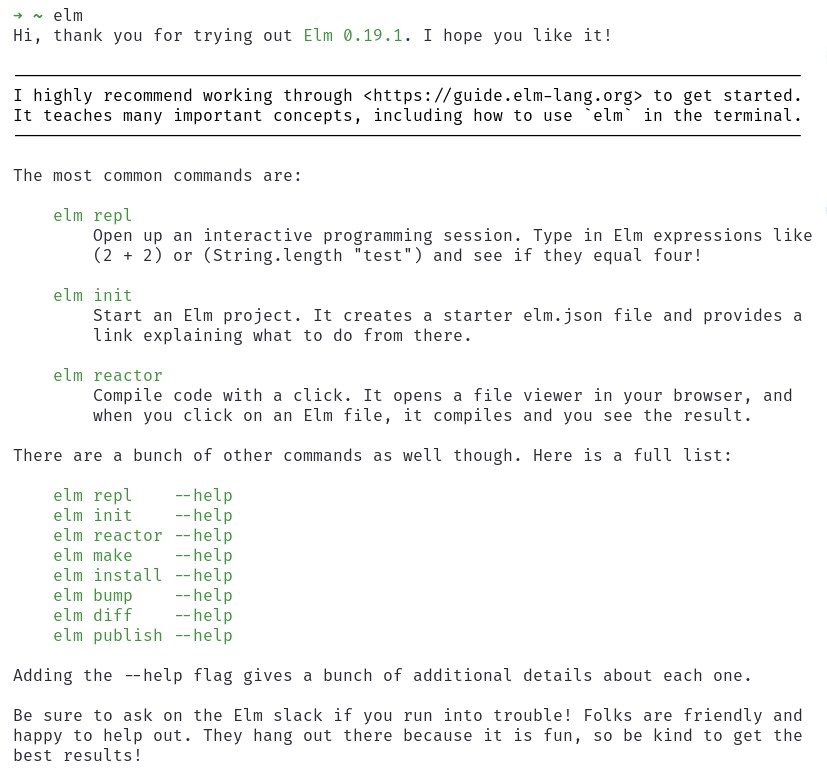
\includegraphics[width=0.95\textwidth]{elm_output.png}
    \caption{Wyjście instrukcji \texttt{elm}}\label{elm_output}
\end{figure}

\subsubsection{Linux}
Najprostszym sposobem instalacji platformy Elm na systemie operacyjnym Linux jest wykorzystanie narzędzia \texttt{npm}~-- powszechnie używanego menadżera pakietów służącego do zarządzania warstwą frontendową aplikacji internetowych.
Aby zainstalować \texttt{npm} należy skorzystać z systemowego menadżera pakietów.
Na przykładzie dystrybucji Ubuntu będą to komendy:
\begin{lstlisting}[language=bash]
  $ sudo apt update
  $ sudo apt install npm
\end{lstlisting}
Kiedy narzędzie zostanie już pomyślnie zainstalowane, można przejść do instalacji platformy Elm.
Posłuży do tego polecenie:
\begin{lstlisting}[language=bash]
  $ npm install -g elm
\end{lstlisting}
Zgodnie z dokumentacją \texttt{npm}~\cite{npmdocs}, flaga \texttt{-g} oznacza, że pakiet zostanie zainstalowany globalnie, dzięki czemu będzie dostępny z każdego miejsca z systemu.
Aby sprawdzić, czy rzeczywiście tak się stało, wystarczy w wierszu poleceń uruchomić komendę \texttt{elm}.
Naszym oczom powinien ukazać się widok podobny do rysunku~\ref{elm_output}, tak jak zostało to już wcześniej wspomniane.
\subsubsection{Windows}
Osoby korzystające z systemu operacyjnego Windows mogą skorzystać z npm, tak jak to było opisane w powyższej sekcji dotyczącej Linuxa lub posłużyć się dedykowanym \href{https://github.com/elm/compiler/releases/download/0.19.1/installer-for-windows.exe}{instalatorem Elm'a}~\cite{elm_installer} na system Windows.
W tym drugim przypadku wystarczy przejść przez wszystkie kroki zostawiając opcje domyślne i w rezultacie Elm zostanie pomyślnie zainstalowany i będzie gotowy do użytkowania.
W celu sprawdzenia czy faktycznie tak się stało, należy uruchomić wiersz poleceń oraz wykonać instrukcję \texttt{elm}. Wyjście komendy powinno być podobne do tego przedstawionego na rysunku~\ref{elm_output}, tak jak zostało to już wcześniej wspomniane.

\subsection{Edytor}
Ważnym elementem tworzenia oprogramowania jest wyposażenie się w odpowiedni edytor tekstowy, który jest w stanie podświetlać składnię języka, z którego aktualnie korzystamy.
Żeby osiągnąć ten cel, w przypadku Elm'a potrzebna będzie instalacja dodatkowej wtyczki do jednego z następujących edytorów:
\begin{itemize}[noitemsep,topsep=0pt]
    \item{\href{https://atom.io/packages/language-elm}{Atom}}
    \item{\href{https://github.com/jcollard/elm-mode}{Emacs}}
    \item{\href{https://github.com/klazuka/intellij-elm}{IntelliJ}}
    \item{\href{https://github.com/rundis/elm-light}{Light Table}}
    \item{\href{https://github.com/evancz/elm-syntax-highlighting/}{Sublime Text}}
    \item{\href{https://github.com/elm-tooling/elm-vim}{Vim}}
    \item{\href{https://github.com/elm-tooling/elm-language-client-vscode}{VS Code}}
\end{itemize}

Powyższa lista zawiera odnośniki do wspomnianych wtyczek dla danego edytora, wystarczy kliknąć nazwę swojego ulubionego edytora i pobrać odpowiedni dodatek.

\subsection{Tworzenie projektu}
Elm jest dostarczany wraz z zestawem bardzo przydatnych narzędzi.
Jednym z nich jest \texttt{elm init}, które posłuży nam do stworzenia nowego projektu.
W tym celu należy otworzyć wiersz poleceń i wykonać następujące instrukcje:

\begin{lstlisting}[language=bash]
  $ mkdir elm_project
  $ cd elm_project
  $ elm init
\end{lstlisting}

Po wypisaniu zawartości katalogu \texttt{elm\_project} z użyciem polecenia \texttt{ls} powinny pojawić się dwa nowe elementy:

\begin{itemize}[noitemsep,topsep=0pt]
    \item{Plik \texttt{elm.json} opisujący projekt oraz jego zależności}
    \item{Katalog \texttt{src/} zawierący nasze przyszłe pliki Elm'a}
\end{itemize}

Następnym krokiem będzie utworzenie nowego pliku \texttt{Main.elm} w nowoutworzonym katalogu \texttt{src/}.
Będzie się tam znajdował kod naszej aplikacji, którą stworzymy w kolejnych krokach.

\section{Podstawy języka Elm}

\subsection{Wartości}

\subsection{Funkcje}

\section{Aplikacja frontendowa}
W ramach większego projektu zbudujemy stronę internetową typu \texttt{startpage}, czyli strony startowej przeglądarki zawierającej najważniejsze i najczęściej używane elementy.
W naszym przypadku będą to cztery moduły -- zegar, pogoda, wyszukiwarka oraz pasek zakładek.

\subsection{Zegar}

\subsection{Pogoda}

\subsection{Wyszukiwarka}

\subsection{Zakładki}

\subsection{Dokument hipertekstowy}
\begin{lstlisting}[caption={Zawartość pliku \texttt{index.html}},language=html]
<head>
    <link rel="stylesheet" href="assets/styles.css" />
    <script src="assets/main.js"></script>
    <script src="assets/bookmarks.js"></script>
</head>
<body>
    <div id="myapp"></div>
    <script>
        var app = Elm.Main.init({
            node: document.getElementById('myapp'),
            flags: bookmarks
        });
    </script>
</body>
\end{lstlisting}

\subsection{Style}

% --------------------------------------------------------------------------------

\chapter{Automatyzacja}
W poniższym rozdziale chciałbym opisać procesy \textit{CI/CD} oraz korzyści płynące z ich używania, a także zaprezententować implementację takich rozwiązań na przykładzie stworzonej wcześniej aplikacji w Elm'ie.

\section{CI/CD}
Mianem CI/CD (Continuous Integration / Continuous Delivery) określa się zbiór praktyk pozwających na ciągłą integrację oraz ciągłe wdrażanie projektów informatycznych.
\begin{figure}[H]
    \centering
    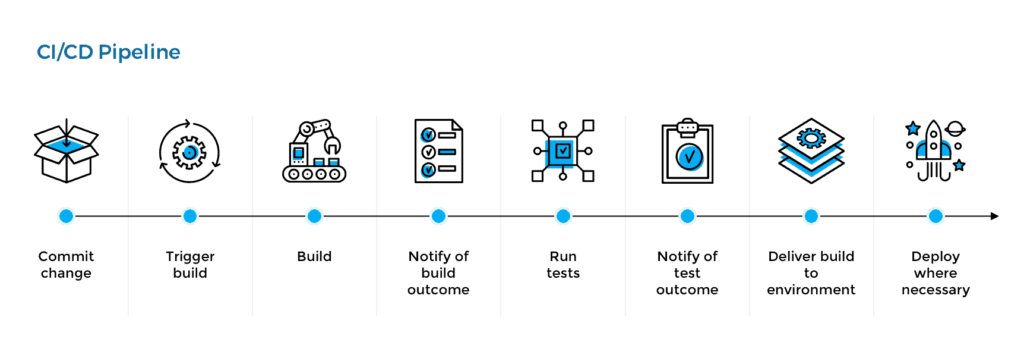
\includegraphics[width=1\textwidth]{cicd_pipeline.png}
    \caption{Przykładowy potok CI/CD}\label{cicd_pipeline}
\end{figure}


\subsection{Ciągła integracja}

\subsection{Ciągłe wdrażanie}

\section{GitHub Actions}

\section{GitHub Pages}

% --------------------------------------------------------------------------------

\chapter{Podsumowanie}

\section{Wnioski}

% --------------------------------------------------------------------------------

\listoffigures
% \listoftables
\lstlistoflistings{}

\printbibliography{}

% --------------------------------------------------------------------------------

\end{document}
